\let\negmedspace\undefined
\let\negthickspace\undefined
\documentclass[journal]{IEEEtran}
\usepackage[a5paper, margin=10mm, onecolumn]{geometry}
%\usepackage{lmodern} % Ensure lmodern is loaded for pdflatex
\usepackage{tfrupee} % Include tfrupee package

\setlength{\headheight}{1cm} % Set the height of the header box
\setlength{\headsep}{0mm}     % Set the distance between the header box and the top of the text

\usepackage{gvv-book}
\usepackage{gvv}
\usepackage{cite}
\usepackage{amsmath,amssymb,amsfonts,amsthm}
\usepackage{algorithmic}
\usepackage{graphicx}
\usepackage{textcomp}
\usepackage{xcolor}
\usepackage{txfonts}
\usepackage{listings}
\usepackage{enumitem}
\usepackage{mathtools}
\usepackage{gensymb}
\usepackage{comment}
\usepackage[breaklinks=true]{hyperref}
\usepackage{tkz-euclide} 
\usepackage{listings}
% \usepackage{gvv}                                        
\def\inputGnumericTable{}                                 
\usepackage[latin1]{inputenc}                                
\usepackage{color}                                            
\usepackage{array}                                            
\usepackage{longtable}                                       
\usepackage{calc}                                             
\usepackage{multirow}                                         
\usepackage{hhline}                                           
\usepackage{ifthen}                                           
\usepackage{lscape}
\usepackage{pgfplots}
\begin{document}

\bibliographystyle{IEEEtran}
\vspace{3cm}

\title{1-1.5-32}
\author{AI24BTECH11033-Tanishq Rajiv Bhujbale}
% \maketitle
% \newpage
% \bigskip
{\let\newpage\relax\maketitle}

\renewcommand{\thefigure}{\theenumi}
\renewcommand{\thetable}{\theenumi}
\setlength{\intextsep}{10pt} % Space between text and floats


\numberwithin{equation}{enumi}
\numberwithin{figure}{enumi}
\renewcommand{\thetable}{\theenumi}


\textbf{Question}:\\
Find the ratio in which the line segment joining the points $\brak{1,-3}$ and $\brak{4, 5}$ is divided by $X$ axis.

\textbf{Solution}:\\

\renewcommand{\tablename}{TABLE 1}
\begin{table}[h!]    
  \centering
  \begin{tabular}{|c|c|}
\hline
\textbf{points} & \textbf{values}\\
\hline
\textbf{A} & $\myvec{1\\-3}$\\
\hline
\textbf{B} & $\myvec{4\\5}$\\
\hline
\textbf{C} & $\myvec{x\\0}$\\
\hline
\end{tabular}

  \caption{values of the geometrical points in given question}
  \label{tab1-1.2-18-1}
\end{table}


If C divides AB in the ratio k : 1


\begin{align}
C=\frac{kB+A}{k+1}
\end{align}

  Substituting A ,B and C in the formula 
  
 \begin{align} 
 \myvec{ \frac{4.k+1}{k+1}\\ \frac{k.5-3}{k+1}} = \myvec{ x \\ 0} \\	 
 \frac{k.5-3}{k+1} = 0 \\
 k=\frac{3}{5}=3:5 
\end{align}

\begin{figure}[h!]
   \centering
   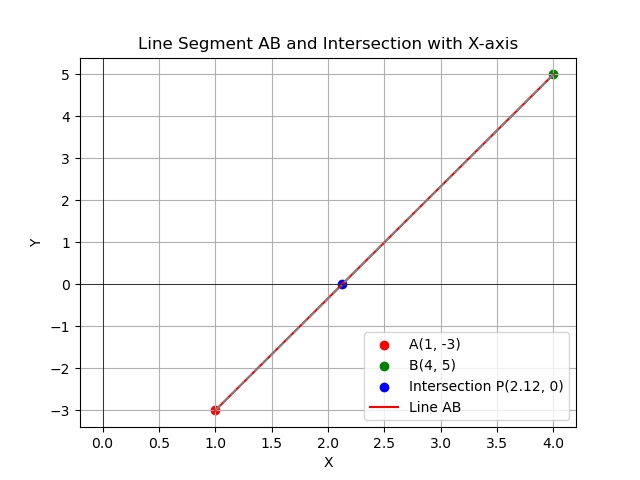
\includegraphics[width=0.7\linewidth]{figs/Figure_1.png}
   \caption{plot for line}
   \label{fig. 1-1.5-32}
\end{figure}


\end{document}
